\chapter{Domain Decomposition}
\label{section:design:domain-decomposition}

Peano 4 starts from spacetrees and thinks in whole trees and only supports two
types of decomposition operations: a split and a join.
At the same time, it does not distinguish shared memory and distributed memory
parallelisation.
It only thinks in terms of trees.
The trees and their traversal can either be deployed to ranks or threads or
combinations of the two.

This statement is only weakened once you work with Peano's task interface. 
If trees issue tasks, then these tasks team up with the tasks handling the
individual spacetrees.
Your task graph starts to contain a mixture of tree tasks and user-defined
tasks.


\section{Multigrid topology}

A tree in Peano is split along the Peano space-filing curve.
This implies that the decomposition of the finest mesh is a non-overlapping
decomposition where each cell is assigned to exactly one rank.
I use rank as term for rank or thread or task. 
See the discussion above.


Also Peano's coarser cells are uniquely assigned to one tree. 
Between the ranks, we have a tree topology again. 
That is, a splitting of a tree is always realised such that there's a unique
master-worker topology.

\begin{figure}
  \begin{center}
    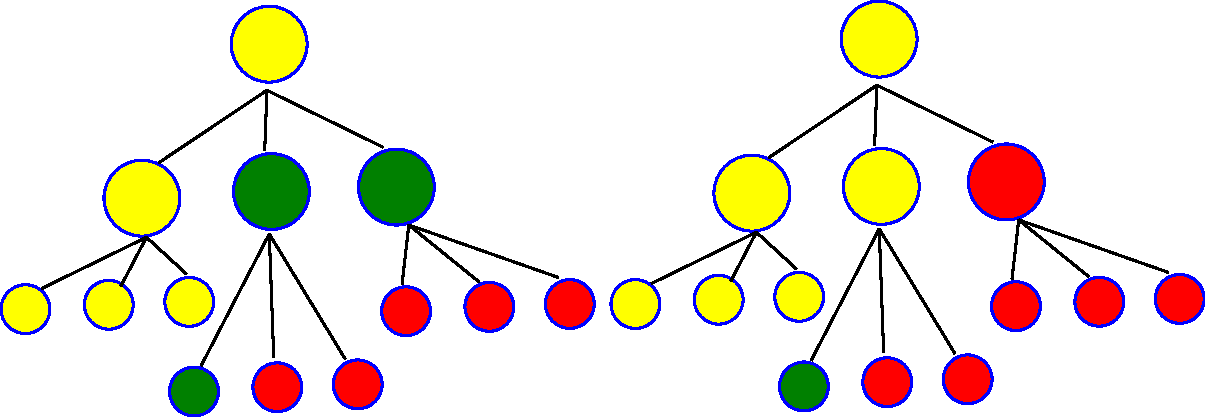
\includegraphics[width=0.8\textwidth]{51_domain-decomposition/tree-topology.pdf}
  \end{center}
  \caption{
    Two examples of a tree decomposition.
    \label{figure:51_domain-decomposition:tree-topology}
  }
\end{figure}

Some examples in Figure \ref{figure:51_domain-decomposition:tree-topology}
sketch the implications:
In the left example, the yellow tree has split up into yellow and green. The
green tree has further split into green and red.
The code usually tries to keep whole trees, i.e.~children and parents, within
one tree.
In the left example, it would be natural to make the very right green cell on
the first child level a red one, too.
This way, a whole tree would reside in red.
However, if we made this single cell red, then red would become a child of
yellow, i.e.~we would change the rank topology.
Peano never does so.

In the right example conversely, I've asked the yellow tree to split into
yellow, green and red in one rush. 
This time, the right level 1 cell becomes red already. 

Both examples show that a split of one tree into $n$ trees never
results in the fact that the original tree becomes empty.
Otherwise, we woudl again change the tree topology upon the ranks.


\section{Splits}

Whenever you split a tree, Peano creates the new trees (either as threads on
the local node or remotely via MPI). 
Each new tree receives a whole copy of the original tree. 
Yes, a whole copy including all user data used within the currently active
sweep.
Once all data is replicated, the individual trees start to coarsen.
If they are not responsible for tree parts, they successively remove this part. 
After one or two iterations, each rank thus really works only on local data plus
all the data that is required to make the locally stored data a real tree.


\begin{remark}
 Peano uses information from the actively used data to decide which data to
 replicate.
 If you have cell and vertex and face data but you use some of these data only
 in some substeps of you algorithm, please ensure that those steps that trigger
 the domain decomposition and those that run immediately after this do use all
 data types.
 Otherwise, Peano can't know what data is to be replicated when it splits trees.
\end{remark}


\section{Joins}

Joins are completely hidden from the user, i.e.~there's no way to actively join
trees. 
To understand why Peano issues joins from time to time, it is important to
define vetoed coarsening.

\begin{definition}
 Peano vetos any coarsening, if removing some parts of the grid would affect a
 child or alter the tree topology of the ranks.
 If a coarsening is vetoed, Peano remembers this veto. 
 As soon as a rank whose master is affected by a veto hosts a tree cell which is
 unrefined, it joins/merges this cell into the master.
\end{definition}

\noindent
Vetoed coarsening typically does delay any grid coarsening.
You ask for a coarsened grid, and it first of all applies this coarsening to all
ranks that have not decomposed further.
Once these have finished their coarsening, it joins those ranks that stop
further coarsening into their master.
Once this is complete, it continues to coarsen.
This process can continue recursively.


\section{Grid entity markers}

As pointed out above, Peano works with replica of trees and then removes per
rank those grid entites which are not adjacent to the local domain.
This implies that some cells plus their data are held redundantly.

Whenever Peano invokes an activitiy on a grid entity, it passes a marker besides
the actual data.
Markers typically hold spatial information.
In a parallel run, a marker also tells you whether the cell or vertex currently
handled is a local one, adjacent to the domain boundary, or overlaps into a
neighbouring domain which actually holds it.
